\documentclass[border=10pt]{standalone}
\usepackage{pgfplots}
\usepgfplotslibrary{colormaps}
\pgfplotsset{trig format plots=rad}
\begin{document}
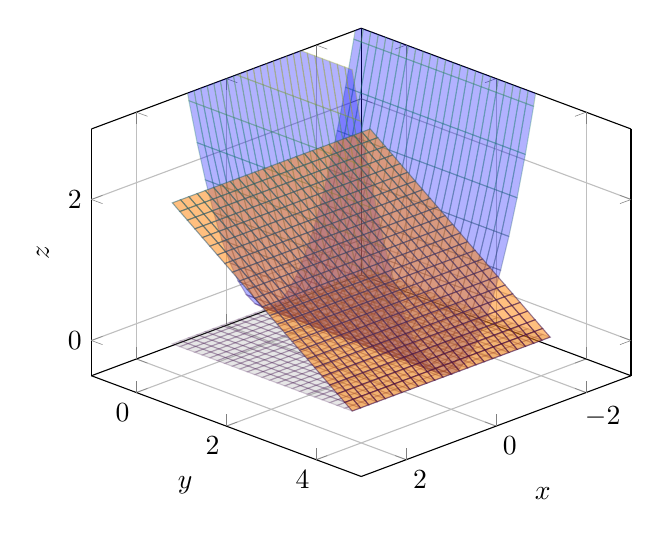
\begin{tikzpicture}
\begin{axis}[
    view={135}{30},
    xlabel=$x$, ylabel=$y$, zlabel=$z$,
    xmin=-3, xmax=3,
    ymin=-1, ymax=5,
    zmin=-0.5, zmax=3,
    grid=both,
    colormap/viridis
]
    % Surface y = x^2
    \addplot3[surf, domain=-2.2:2.2, y domain=0:4, opacity=0.3, blue] {x^2};
    
    % Surface z = 0
    \addplot3[surf, domain=-2.2:2.2, y domain=0:4, opacity=0.2, gray] {0};
    
    % Surface y + 2z = 4 => z = (4-y)/2
    \addplot3[surf, domain=-2.2:2.2, y domain=0:4, opacity=0.5, orange] {(4-y)/2};
    
\end{axis}
\end{tikzpicture}
\end{document}
